%%%%%%%% ICML 2023 EXAMPLE LATEX SUBMISSION FILE %%%%%%%%%%%%%%%%%

\documentclass{article}

% Recommended, but optional, packages for figures and better typesetting:
\usepackage{microtype}
\usepackage{graphicx}
\usepackage{pdfpages}
\usepackage{hyperref}
\usepackage{glossaries}
\usepackage{graphicx}
\usepackage{subfigure}
\usepackage{booktabs} % for professional tables
\usepackage{float}

\usepackage{tikz}
% Corporate Design of the University of Tübingen
% Primary Colors
\definecolor{TUred}{RGB}{165,30,55}
\definecolor{TUgold}{RGB}{180,160,105}
\definecolor{TUdark}{RGB}{50,65,75}
\definecolor{TUgray}{RGB}{175,179,183}

% Secondary Colors
\definecolor{TUdarkblue}{RGB}{65,90,140}
\definecolor{TUblue}{RGB}{0,105,170}
\definecolor{TUlightblue}{RGB}{80,170,200}
\definecolor{TUlightgreen}{RGB}{130,185,160}
\definecolor{TUgreen}{RGB}{125,165,75}
\definecolor{TUdarkgreen}{RGB}{50,110,30}
\definecolor{TUocre}{RGB}{200,80,60}
\definecolor{TUviolet}{RGB}{175,110,150}
\definecolor{TUmauve}{RGB}{180,160,150}
\definecolor{TUbeige}{RGB}{215,180,105}
\definecolor{TUorange}{RGB}{210,150,0}
\definecolor{TUbrown}{RGB}{145,105,70}


\newacronym{BW}{BW}{Baden-Württemberg}
\newacronym{NRW}{NRW}{Nordrhein-Westphalia}
\newacronym[shortplural=SD, firstplural=standard deviations (SD)]{SD}{SD}{standard deviation}
\newacronym{RBF}{RBF}{Radial basis function}
% hyperref makes hyperlinks in the resulting PDF.
% If your build breaks (sometimes temporarily if a hyperlink spans a page)
% please comment out the following usepackage line and replace
% \usepackage{icml2023} with \usepackage[nohyperref]{icml2023} above.
\usepackage{hyperref}


% Attempt to make hyperref and algorithmic work together better:
\newcommand{\theHalgorithm}{\arabic{algorithm}}

\usepackage[accepted]{icml2023}

% For theorems and such
\usepackage{amsmath}

\usepackage{amssymb}
\usepackage{svg}
\usepackage{mathtools}
\usepackage{amsthm}
\usepackage{booktabs} % For better-looking tables
\usepackage{caption}  % For adjusting caption style
\usepackage{adjustbox} % For adjusting table wid
% if you use cleveref..
\usepackage[capitalize,noabbrev]{cleveref}

%%%%%%%%%%%%%%%%%%%%%%%%%%%%%%%%
% THEOREMS
%%%%%%%%%%%%%%%%%%%%%%%%%%%%%%%%
\theoremstyle{plain}
\newtheorem{theorem}{Theorem}[section]
\newtheorem{proposition}[theorem]{Proposition}
\newtheorem{lemma}[theorem]{Lemma}
\newtheorem{corollary}[theorem]{Corollary}
\theoremstyle{definition}
\newtheorem{definition}[theorem]{Definition}
\newtheorem{assumption}[theorem]{Assumption}
\theoremstyle{remark}
\newtheorem{remark}[theorem]{Remark}

% Todonotes is useful during development; simply uncomment the next line
%    and comment out the line below the next line to turn off comments
%\usepackage[disable,textsize=tiny]{todonotes}
\usepackage[textsize=tiny]{todonotes}


% The \icmltitle you define below is probably too long as a header.
% Therefore, a short form for the running title is supplied here:
\icmltitlerunning{Project Report Template for Data Literacy 2023/24}

\begin{document}
\twocolumn[
\icmltitle{Analyzing Network Stability along Germany's Long-Distance Rail Network: \\A Comparison of North Rhine-Westphalia and Baden-Wuerttemberg}

%Analyzing Mobile Network Stability along Deutsche Bahn's Long-Distance Rail Networks: A Comparison of North Rhine-Westphalia and Baden-Wuerttemberg

%Comparative Analysis of Internet Stability among Providers in Deutsche Bahn: A Case Study of Baden-Württemberg and North Rhine-Westphalia

% It is OKAY to include author information, even for blind
% submissions: the style file will automatically remove it for you
% unless you've provided the [accepted] option to the icml2023
% package.

% List of affiliations: The first argument should be a (short)
% identifier you will use later to specify author affiliations
% Academic affiliations should list Department, University, City, Region, Country
% Industry affiliations should list Company, City, Region, Country

% You can specify symbols, otherwise they are numbered in order.
% Ideally, you should not use this facility. Affiliations will be numbered
% in order of appearance and this is the preferred way.
\icmlsetsymbol{equal}{*}

\begin{icmlauthorlist}
\icmlauthor{Jonas Fluck}
{equal,first}
\icmlauthor{David Grimm}
{equal,second}
\icmlauthor{Julius Braitinger}
{equal,third}
\end{icmlauthorlist}

% fill in your matrikelnummer, email address, degree, for each group member
\icmlaffiliation{first}{Matrikelnummer 6758981, Jonas.Fluck@student.uni-tuebingen.de, MSc Medical Informatics}
\icmlaffiliation{second}{Matrikelnummer 6758006, David.Grimm@student.uni-tuebingen.de, MSc Medical Informatics}
\icmlaffiliation{third}{Matrikelnummer 6759173, Julius.Braitinger@student.uni-tuebingen.de, MSc Medical Informatics}


% You may provide any keywords that you
% find helpful for describing your paper; these are used to populate
% the "keywords" metadata in the PDF but will not be shown in the document
\icmlkeywords{Machine Learning, ICML}

\vskip 0.3in
]

% this must go after the closing bracket ] following \twocolumn[ ...

% This command actually creates the footnote in the first column
% listing the affiliations and the copyright notice.
% The command takes one argument, which is text to display at the start of the footnote.
% The \icmlEqualContribution command is standard text for equal contribution.
% Remove it (just {}) if you do not need this facility.

%\printAffiliationsAndNotice{}  % leave blank if no need to mention equal contribution
\printAffiliationsAndNotice{\icmlEqualContribution} % otherwise use the standard text.

\begin{abstract}
In an era defined by constant connectivity, seamless mobile network coverage is vital, especially during travel. The following project report investigates the mobile network stability in Germany along Deutsche Bahn's long-distance rail network in the federal states of Baden-Wuerttemberg and North Rhine-Westphalia. This analysis of  major network provider's stability used a comprehensive dataset and a Gaussian process to estimate missing data points. The findings reveal slight variations in stability metrics across providers and regions, with Vodafone emerging as the most reliable option. However, it's important to note that the age of the data and the amount of missing data points limit definitive conclusions.
\end{abstract}
\section{Introduction}\label{sec:intro}
In 2023, Deutsche Bahn AG's long-distance transport service attracted 132 million passengers \citep{deutschebahn2022}. When traveling by train and wanting to maximize travel time utility, seamless mobile network availability is crucial. This paper examines the stability of mobile networks along the long-distance rail network in Germany, with a focus on the federal states of \gls*{BW} and \gls*{NRW}. The investigation aims to identify the most reliable network provider among T-Mobile, Vodafone, o2, and e-plus.  To enhance the integrity of the data, missing measurements were estimated using a Gaussian process regression, which is described in more detail in the Data and Methods section. The findings are presented through visualizations and an interactive map of Germany, accessible on \href{https://github.com/JonasFluck/DBNet.git}{GitHub}.

%\Motivate the problem, situation or topic you decided to work on. Describe why it matters (is it of societal, economic, scientific value?). Outline the rest of the paper (use references, e.g.~to \Cref{sec:methods}: What kind of data you are working with, how you analyse it, and what kind of conclusion you reached. The point of the introduction is to make the reader want to read the rest of the paper.
\section{Data and Methods}\label{sec:methods}
The dataset, sourced from Deutsche Bahn \citep{db-netzradar}, consists of segments of rail network, organized by latitude and longitude coordinates divided into 500-meter sections. The dataset is structured as a GeoJSON FeatureCollection. These features are defined as LineString geometries that outline the coordinates of a track. Properties within each feature include measurements of mobile network stability from 2016, distinguishing between different network providers (T-Mobile, Vodafone, e-plus, o2) and network technologies (with or without 4G). 
 \begin{figure}[H]
 \vskip 0.2in
 \begin{center}
\centerline{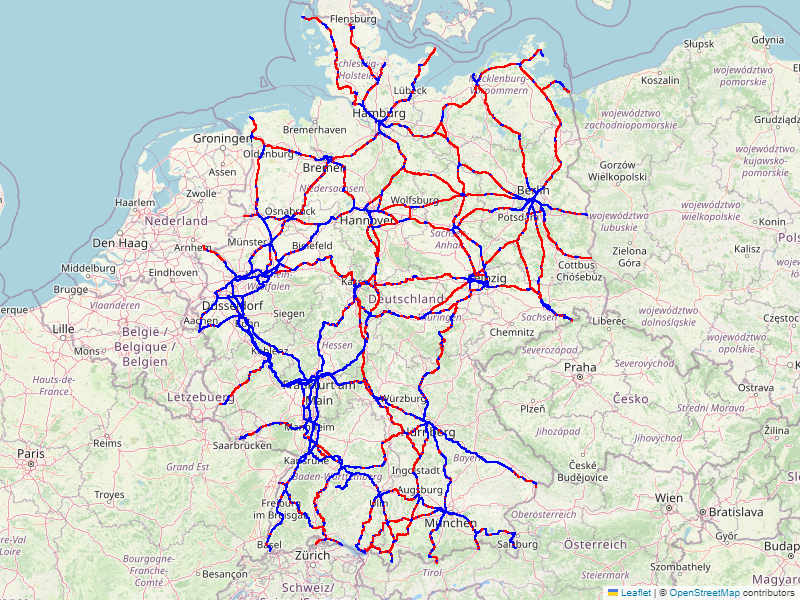
\includegraphics[width=\columnwidth]{EmptyStabilityMap.png}}
\caption{Map of Germany with the long-distance railway lines, color-coded to indicate the presence of measurements. Red indicates routes without measurements. Blue indicates routes with measurements.}
 \label{fig:mapGauss}
 \end{center}
 \vskip -0.2in
 \end{figure} 
The stability of a track is defined as a value between zero and one, which represents the percentage of measurements in which an internet connection was established.
We focused solely on the measurements and the stability attribute without considering the non 4G-related metrics. 
There are a total of 23~727 different 500-meter tracks, with  4~113~130 overall measurements. There is a significant variation in the number of measurements taken by different providers. Vodafone recorded the most measures with a total of 2~482~426, followed by T-Mobile with 744~406 measurements, e-plus with 490~806, and o2 with 304~071.
\newline
We decided on developing a Streamlit application as an interactive tool for better exploration of the data.
For visualizing the raw data itself, we created an interactive map using the folium library in Python (see \hyperref[fig:mapGauss]{Figure 1})
The map, centered on Germany and based on OpenStreetMap \citep{OpenStreetMap}, displays each track's coordinates. Stability values are represented using a color-blind-friendly scale, transitioning from orange to blue. Orange indicates poor stability, while blue indicates good stability.
\newline
\\
Due to the high number of missing data points in various federal states, we focused on two of them for the comparison: \gls*{BW} and \gls*{NRW}. Both have a significant quantity of measurements. In \gls*{BW}, there are a total of 2~713 data points, resulting in a coverage rate of 72\%. In \gls*{NRW}, there are 2~810 data points with a measurement coverage rate of 82\%. In other federal states, either the coverage rates or the quantity of data points is lower.
\begin{table*}[htbp]
\centering
\caption{Stability Metrics for Mobile Service Providers in \gls*{BW}}
\label{tab:stability_metrics_bw}
\begin{adjustbox}{width=\textwidth}
\begin{tabular}{@{}lllll@{}}
\toprule
\textbf{Provider} & \textbf{Mean Stability} & \textbf{Mean Uncertainty (SD)} & \textbf{Observed Values} & \textbf{Predicted Values} \\
\midrule
\textbf{\gls*{BW}} & 0.912 & 0.020 & 1953  (71.99\%) & 760 \\
Vodafone & 0.949 & 0.002 & 1361 (50.17\%) & 1352 \\
T-Mobile & 0.892 & 0.073 & 874 (32.22\%) & 1839 \\
e-plus & 0.882 & 0.162 & 509 (18.76\%) & 2204 \\
o2 & 0.840 & 0.217 & 677 (24.95\%) & 2036 \\
\bottomrule
\end{tabular}
\end{adjustbox}
\end{table*}
\begin{table*}[htbp]
\centering
\caption{Stability Metrics for Mobile Service Providers in \gls*{NRW}}
\label{tab:stability_metrics_nrw}
\begin{adjustbox}{width=\textwidth}
\begin{tabular}{@{}lllll@{}}
\toprule
\textbf{Provider} & \textbf{Mean Stability} & \textbf{Mean Uncertainty (SD)} & \textbf{Observed Values} & \textbf{Predicted Values} \\
\midrule
\textbf{\gls*{NRW}} & 0.939 & 0.022 & 2313 (82.31\%) & 497 \\
Vodafone & 0.952 & 0.002 & 1867 (66.44\%) & 943 \\
T-Mobile & 0.918 & 0.071 & 1525 (54.27\%) & 1285 \\
e-plus & 0.889 & 0.136 & 1040 (37.01\%) & 1770 \\
o2 & 0.922 & 0.186 & 1141 (40.60\%) & 1669 \\
\bottomrule
\end{tabular}
\end{adjustbox}
\end{table*}
The original dataset does not provide federal state-specific information. In order to compare the data between BW and NRW, we needed to map each train track to the federal state in which it is located. To achieve this we used an additional GeoJSON file \citep{deutschlandGeoJSON} containing coordinates that outline each federal state as a multipolygon. We then mapped each track to the corresponding state and added a column to each data point which contains the affiliation to a certain federal state.
\newline
\\
To manage the large quantity of data points where no measurements were taken, a K-nearest-neighbor (KNN) approach first seemed like the simplest method for solving the problem. However, this approach did not provide a measure of uncertainty associated with the computed predictions. Given the quantity of missing data, uncertainty appeared to be meaningful in terms of the predicted data. 
\newline
\\
A Gaussian process regression, on the other hand, offers the possibility of measuring the uncertainty of predictions in \glspl*{SD}, so we decided to use this approach to estimate the missing stability values. First, we needed to find the appropriate hyperparameters and kernel function to run the Gaussian process regression. To determine the best fit, we ran a random search on both a Matern and a \gls*{RBF} kernel with 80\% of all data provided as training data and 20\% as test data. As a result of a five-fold cross-validation, an RBF kernel, which had the lowest mean squared error, was subsequently used for all predictions of missing stability values, both overall and provider-specific. The implementation of the Gaussian process regression was facilitated by the functionalities provided by the scikit-learn package \citep{scikit-learn}. The predicted values for the missing stability data, along with the uncertainties associated with these predictions, were then incorporated into the dataset for further analysis (\hyperref[fig:confidence]{Figure 2}).
\begin{figure}[H]
\vskip 0.2in
\begin{center}
\centerline{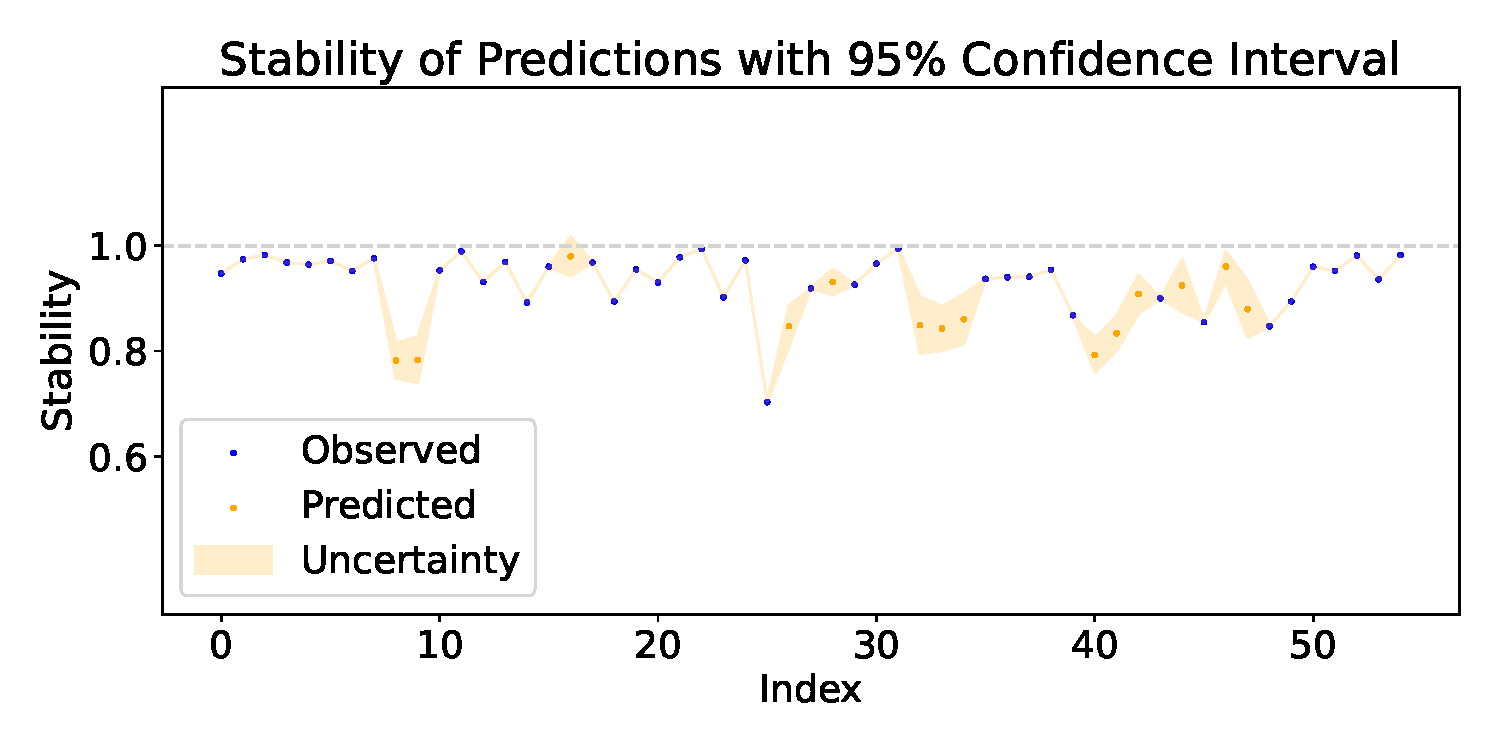
\includegraphics[width=\columnwidth]{gauss.pdf}}
\caption{The graph shows stability values for \gls*{BW}, observed in blue and predicted in orange, with shaded regions indicating 95\% confidence intervals around predicted points. 
To enhance readability, only every 50th stability value is displayed. The y-axis represents stability values ranging from zero to one. The x-axis denotes data point indices.}
\label{fig:confidence}
\end{center}
\vskip -0.2in
\end{figure}
The means for each network provider were then calculated using the data for the specific federal states of \gls*{BW} and \gls*{NRW}, which also included the estimated predictions.
\\
\newline
To validate the results, it is important to check whether the stability value correlates with the number of measurements. A chi-square test of independence was conducted to determine a correlation between the two categorical variables 'presence of at least one measurement' which can be categorized as true or false, and 'stability category is 80-100\%'. Especially the hypothesis H\textsubscript{0}: There is no relationship between the variable 'isMeasured' and the stability category '80-100\%' will be investigated. For this test we subdivided the whole dataset into five categories, which are represented as 20\% intervals.\\
In addition, the relationship between the number of measurements and the stability rate was investigated through the Pearson correlation (\hyperref[fig:pearson]{Figure 4}).
 %If you downloaded data from the net, show an exploratory analysis that builds intuition for the data, and shows that you know the data well. If you are doing a custom analysis, explain how it works and why it is the right choice. If you are using a standard tool, it may still help to briefly outline it. Cite relevant works. You can use the \verb|\citep| and \verb|\citet| commands for this purpose \citep{mackay2003information}.
% This is the template for a figure from the original ICML submission pack. In lecture 10 we will discuss plotting in detail.
% Refer to this lecture on how to include figures in this text.
% 
% \begin{figure}[ht]
% \vskip 0.2in
% \begin{center}
% \centerline{\includegraphics[width=\columnwidth]{icml_numpapers}}
% \caption{Historical locations and number of accepted papers for International
% Machine Learning Conferences (ICML 1993 -- ICML 2008) and International
% Workshops on Machine Learning (ML 1988 -- ML 1992). At the time this figure was
% produced, the number of accepted papers for ICML 2008 was unknown and instead
% estimated.}
% \label{icml-historical}
% \end{center}
% \vskip -0.2in
% \end{figure}
\newpage
\section{Results}\label{sec:results}
%The mean stability over all providers is 0.912 in BW, which is based on 1~953 observed and 760 predicted values. For Vodafone the mean stability is 0.949 with a mean uncertainty for the predicted stability values of 0.002 standard deviations. T-mobile shows a mean stability of 0.892 where the mean uncertainty is around 0.073 standard deviations. e-plus and o2 have a mean stability of 0.882 (mean uncertainty of 0.162 standard deviations) and 0.840 (mean uncertainty of 0.217 standard deviations), respectively. This calculations are based on 1361 observed (50.17\%) and 1~352 predicted stabilites for Vodafone, 874 observed (32.22\%) and 1~839 predicted stabilites for T-Mobile. e-plus has 509 observed (18.76\%) and 2~204 predicted stabilities and at least o2 with 677 osberved (24.95\%) and 2~036 predicted stabilities.
%The mean stability across all providers in NRW is 0.939, derived from 2~313 observed and 497 predicted values. Vodafone exhibits an average stability of 0.952, with a mean uncertainty for the predicted stability values of 0.002 standard deviations. T-Mobile demonstrates a mean stability of 0.918, accompanied by a mean uncertainty of approximately 0.071 standard deviations. Conversely, e-plus and o2 showcase mean stabilities of 0.889 and 0.922 with corresponding mean uncertainties of 0.136 and 0.186 standard deviations, respectively.
%These calculations are based on 1,867 observed and 943 predicted stabilities for Vodafone, 1,525 observed and 1,285 (54.27\%) predicted stabilities for T-Mobile, 1,040 observed and 1,770 (37.01\%) predicted stabilities for e-plus, and 1,141 observed and 1,669 (40.60\%) predicted stabilities for o2. 
%Through the process of exploring the data, we have developed a Streamlit application that can be used for further analysis and comparison.
There is a small difference in overall stability between \gls*{BW} and \gls*{NRW}, with a noticeable variance in stability means among providers. In both federal states, Vodafone has the best stability mean as well as the most measurements of stability values. It is observable that o2 has the highest difference in stability means among the providers with a mean stability of 0.922 in \gls*{NRW}, and 0.840 in \gls*{BW}, which are simultaneously the values associated with the highest uncertainty. It is noticeable that the uncertainty varies between different providers and is in general slightly higher in \gls*{BW} than in \gls*{NRW} for both the entire federal state and the different providers (\hyperref[tab:stability_metrics_bw]{Table 1} and \hyperref[tab:stability_metrics_nrw]{Table 2}). 
 \begin{figure}[H]
 \begin{center}
\centerline{\includesvg[width=\columnwidth]{provider_comparison.svg}}
\caption{The bar chart shows the average stability percentages for the four provider. The black bar represents the average of all observed values, while the gray bar represents the mean including predicted data.}
 \label{fig:barchart}
 \end{center}
 \end{figure}
In general, the observed stability is greater than predictions by a small amount. The stability means in NRW are more closely spaced, and overall, all of the providers display higher values than in BW (\hyperref[fig:barchart]{Figure~3}).
\\
The result of the chi-square test of independence between 'presence of at least one measurement' and 'stability category is 80 to 100\%' is 15.68 and is associated with a p-value of 6.82e-05. The Pearson correlation test shows a correlation coefficient of 0.018 and a p-value of 0.035, while only the actually observed data poi<nts were considered.
Most of the data points are associated with high stability and a low number of measurements (\hyperref[fig:Pearson]{Figure 4}). On the other hand, values with low stability and a high number of measurements seem to be very sparse.
\section{Discussion \& Conclusion}\label{sec:conclusion}
When looking at the different providers Vodafone emerges as the best choice in both federal states with an above-average stability associated with a low uncertainty of 0.002. 
The other providers also achieve good stability rates, all being above 0.80. o2 has the highest uncertainty among providers in both federal states. This could be due to a large quantity of predicted values and therefore a lower number of observed values, as well as a high variety in the stability rates.
\begin{figure}[H]
\vskip 0.2in
\begin{center}
\centerline{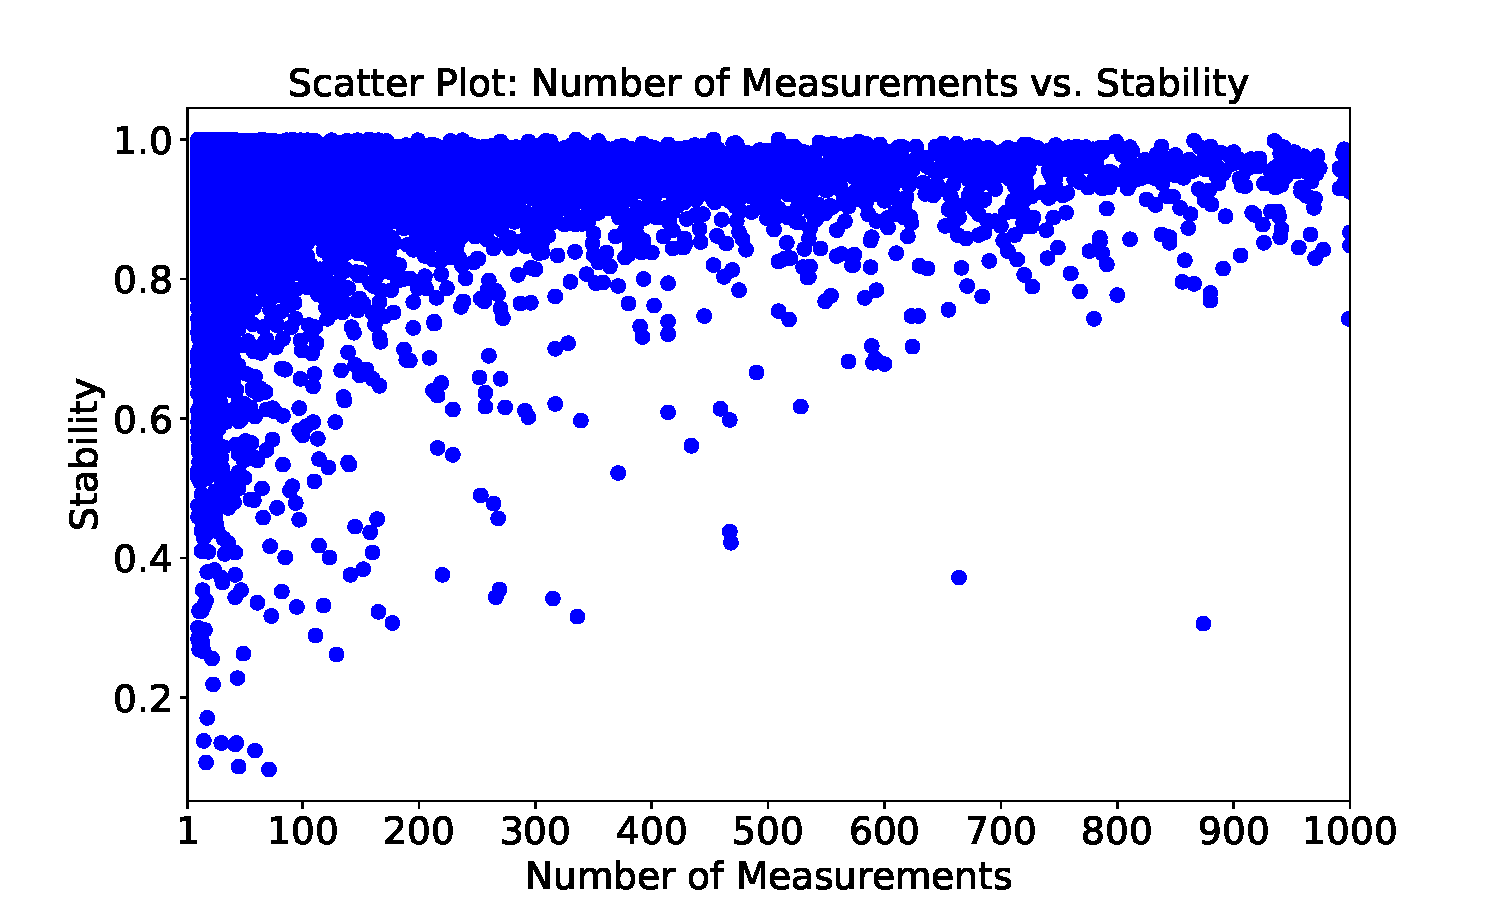
\includegraphics[width=\columnwidth]{measurementStability.pdf}}
\caption{Pearson correlation analysis investigating the relationship between the number of measurements (x-axis) and the stability rate (y-axis), showing only the section from 0 to 1000 measurements}
\label{fig:pearson}
\end{center}
\vskip -0.2in
\end{figure}
However, depending on the number of observed data points the results of the chi-square test of independence are likely to influence the results of the providers. With the previously mentioned hypothesis H\textsubscript{0} and a p-value of 6.82e-05 indicating that it is highly unlikely for H\textsubscript{0} to be true. Therefore, we can reject H\textsubscript{0} in favor of H\textsubscript{1}: There is a relationship between the variable 'isMeasured' and the stability category '80-100\%'. So it can be assumed that the results are biased towards providers with a higher number of data points where at least one measurements was recorded.
\\
The Pearson correlation suggests a slightly positive association between the number of measurements and the stability value. This may be due to the network situation being as good as it appears, or to biased decision-making regarding which measurements were taken.\\
\\
Additionally, the hyperparameters found in the random
search may not be the most fitting for the provided scenario.
It should be noted that other kernels, such as the matern
kernel, may also lead to similar or better results when
provided with more complete data, which could also make
KNN is a viable option again.
\\
\newline
The significant amount of missing data poses a major challenge in making accurate statements. Our approach of predicting the values lead mostly to stability values above 0.8 for the whole of Germany (\hyperref[fig:stability-map]{Figure 5}). It is important to note that these values are influenced by the prevalence of the high observed stability values, so our predictions tend to reflect similarly high values. Another challenge is the age of the dataset, dating back to 2016. Although the data provided by Deutsche Bahn is valuable, a more recent dataset is eagerly anticipated. Germany has witnessed notable advancements in internet stability over the last nine years, including initiatives such as the government's 'Breitbandausbau' project \citep{bundesnetzagentur}. Without current data, it is near impossible to conclusively determine which internet provider performs the best.
\begin{figure}[H]
 \vskip 0.2in
 \begin{center}
\centerline{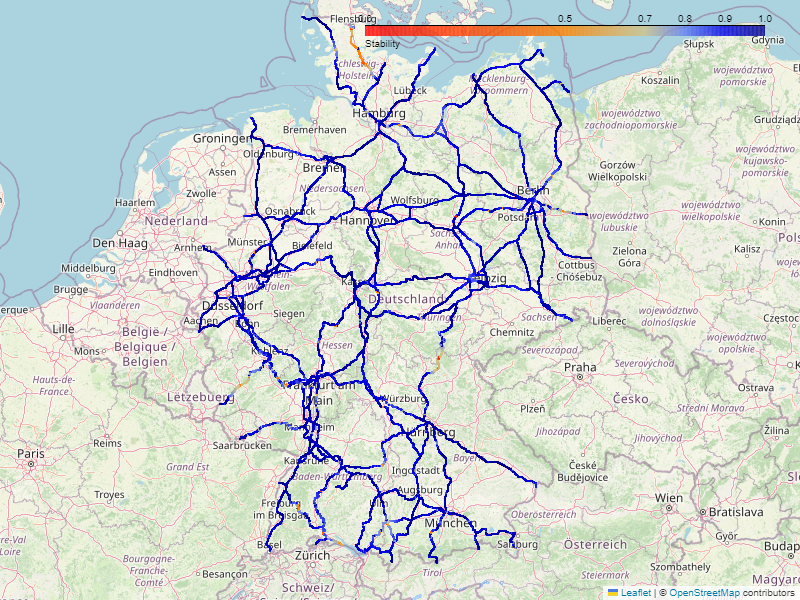
\includegraphics[width=\columnwidth]{StabilityGauss.png}}
\caption{Map of Germany's long-distance railway tracks color-coded to show stability: red (poor) to blue (good).}
 \label{fig:stability-map}
 \end{center}
 \vskip -0.2in
 \end{figure}
In conclusion, this analysis provides insight into the stability of mobile networks along Deutsche Bahn's long-distance rail networks in Baden-Wuerttemberg and North Rhine-Westphalia. The data suggests that Vodafone is the most stable provider, while uncertainties remain, especially with the low count of o2 measurements. However, it is worth noting that the analysis may be affected by missing data and the age of the dataset, highlighting the need for more recent and comprehensive data to draw conclusive insights. Future studies should prioritize updating the underlying datasets to enhance accuracy of possible findings.
%Use this section to briefly summarize the entire text. Highlight limitations and problems, but also make clear statements where they are possible and supported by the analysis. 
\section*{Contribution Statement}
Jonas Fluck was responsible for leading the development of the Streamlit application, implementing map visuals and the Gaussian process regression. Julius Braitinger was responsible for data cleaning, applying the geometry filter, and writing. David Grimm contributed to creating plots, conducting correlation tests, and writing sections. All team members shared equal responsibility for the report.
\newpage
\bibliography{bibliography}
\bibliographystyle{icml2023}

\end{document}


% This document was modified from the file originally made available by
% Pat Langley and Andrea Danyluk for ICML-2K. This version was created
% by Iain Murray in 2018, and modified by Alexandre Bouchard in
% 2019 and 2021 and by Csaba Szepesvari, Gang Niu and Sivan Sabato in 2022.
% Modified again in 2023 by Sivan Sabato and Jonathan Scarlett.
% Previous contributors include Dan Roy, Lise Getoor and Tobias
% Scheffer, which was slightly modified from the 2010 version by
% Thorsten Joachims & Johannes Fuernkranz, slightly modified from the
% 2009 version by Kiri Wagstaff and Sam Roweis's 2008 version, which is
% slightly modified from Prasad Tadepalli's 2007 version which is a
% lightly changed version of the previous year's version by Andrew
% Moore, which was in turn edited from those of Kristian Kersting and
% Codrina Lauth. Alex Smola contributed to the algorithmic style files.
